\documentclass[12pt, a4paper]{article}
\usepackage[utf8]{inputenc}
\usepackage[legalpaper, margin=1in]{geometry}
\usepackage{graphicx}
\usepackage{hyperref}
\usepackage[table]{xcolor}
\usepackage{amsmath}
\usepackage{amssymb}
\usepackage{indentfirst}
\usepackage{pdfpages}
\usepackage{listings}
\usepackage{color}

\definecolor{dkgreen}{rgb}{0,0.6,0}
\definecolor{gray}{rgb}{0.5,0.5,0.5}
\definecolor{mauve}{rgb}{0.58,0,0.82}

\lstset{frame=tb,
  language=Python,
  aboveskip=3mm,
  belowskip=3mm,
  showstringspaces=false,
  columns=flexible,
  basicstyle={\small\ttfamily},
  numbers=none,
  numberstyle=\tiny\color{gray},
  keywordstyle=\color{blue},
  commentstyle=\color{dkgreen},
  stringstyle=\color{mauve},
  breaklines=true,
  breakatwhitespace=true,
  tabsize=3
}

\title{HW1 Clustering and Regression}
\author{6332032921 Pisitpong Chongpipattanakul}
\addtocontents{toc}{\protect\hypertarget{toc}{}}
\sloppy

\renewcommand*{\arraystretch}{1.5}
\begin{document}

\maketitle
\tableofcontents
\noindent\makebox[\linewidth]{\rule{\linewidth}{0.2pt}}

\pagebreak
\section{Metric}

\begin{center}
    \begin{tabular}{| m{5em} | m{7em} | m{7em} |} 
        \hline
        Model A & Predicted dog & Predicted cat \\
        \hline\hline
        Actual dog & 30 & 20 \\ 
        \hline
        Actual cat & 10 & 40 \\
        \hline
    \end{tabular}
\end{center}

\subsection{T1}

\begin{equation}
    \label{Model A Accuracy}
    \begin{split}
        Model\;A\;Accuracy & = \frac{Correct_{dog} + Correct_{cat}}{All} \\
                            & = \frac{30 + 40}{30 + 20 + 10 + 40} \\
                            & = \frac{70}{100} \\
                            & = 0.7 \\
    \end{split}
\end{equation}

\subsection{T2}

In this problem we will consider cat as class 1 (positive).

\begin{equation}
    \label{Precision Cat}
    \begin{split}
        Precision & = \frac{TP}{TP + FP} \\
                    & = \frac{40}{60} \\
                    & = \frac{2}{3} \\
    \end{split}
\end{equation}

\begin{equation}
    \label{Recall Cat}
    \begin{split}
        Recall & = \frac{TP}{TP + FN} \\
                & = \frac{40}{50} \\
                & = 0.8 \\
    \end{split}
\end{equation}

\begin{equation}
    \label{F1 Cat}
    \begin{split}
        F1\;Score & = 2 \cdot \frac{Recall \cdot Precision}{Recall + Precision} \\
                    & = 2 \cdot \frac{\frac{2}{3} \cdot 0.8}{\frac{2}{3} + 0.8} \\
                    & = 2 \cdot \frac{1.6}{2 + 2.4} \\
                    & = 2 \cdot \frac{1.6}{4.4} \\
                    & = \frac{8}{11}
    \end{split}
\end{equation}

\subsection{T3}

In this problem we will consider dog as class 1 (positive).

\begin{equation}
    \label{Precision Dog}
    \begin{split}
        Precision & = \frac{TP}{TP + FP} \\
                    & = \frac{30}{40} \\
                    & = 0.75 \\
    \end{split}
\end{equation}

\begin{equation}
    \label{Recall Dog}
    \begin{split}
        Recall & = \frac{TP}{TP + FN} \\
                & = \frac{30}{50} \\
                & = 0.6 \\
    \end{split}
\end{equation}

\begin{equation}
    \label{F1 Dog}
    \begin{split}
        F1\;Score & = 2 \cdot \frac{Recall \cdot Precision}{Recall + Precision} \\
                    & = 2 \cdot \frac{0.75 \cdot 0.6}{0.75 + 0.6} \\
                    & = 2 \cdot \frac{0.45}{1.35} \\
                    & = \frac{2}{3}
    \end{split}
\end{equation}

\subsection{T4}

Let's assume that the prediction is scaling in linear trend so value in actual dog will be multiplied by 0.4 and value in actual cat will be multiplied by 1.6

The result classification table after scaling
\begin{center}
    \begin{tabular}{| m{5em} | m{7em} | m{7em} |} 
        \hline
        Model B & Predicted dog & Predicted cat \\
        \hline\hline
        Actual dog & 12 & 8 \\ 
        \hline
        Actual cat & 16 & 64 \\
        \hline
    \end{tabular}
\end{center}

\begin{equation}
    \label{Model B Accuracy}
    \begin{split}
        Model\;B\;Accuracy & = \frac{Correct_{dog} + Correct_{cat}}{All} \\
                            & = \frac{12 + 64}{12 + 8 + 16 + 64} \\
                            & = \frac{78}{100} \\
                            & = 0.78 \\
    \end{split}
\end{equation}

And we assign dog as the positive class

\begin{equation}
    \label{Precision Dog B}
    \begin{split}
        Precision & = \frac{TP}{TP + FP} \\
                    & = \frac{12}{12 + 16} \\
                    & = \frac{3}{7} \\
    \end{split}
\end{equation}

\begin{equation}
    \label{Recall Dog B}
    \begin{split}
        Recall & = \frac{TP}{TP + FN} \\
                & = \frac{12}{20} \\
                & = 0.6 \\
    \end{split}
\end{equation}

\begin{equation}
    \label{F1 Dog B}
    \begin{split}
        F1\;Score & = 2 \cdot \frac{Recall \cdot Precision}{Recall + Precision} \\
                    & = 2 \cdot \frac{\frac{3}{7} \cdot 0.6}{\frac{3}{7} + 0.6} \\
                    & = 2 \cdot \frac{1.8}{7.2} \\
                    & = 0.5
    \end{split}
\end{equation}

We see that only recall value remains unchanged but F1 score and precision are changed because ratio between class 1 and class 0 are changed 
so the value of F1 score and precision which also reference to class 0 also have affected

\subsection{OT1}

First, we will reform the equation of Accuracy and F1 Score

\begin{equation}
    \label{Accuracy OT1}
    \begin{split}
        Accuracy & = \frac{TP + TN}{TP + TN + FP + FN} \\
                & = \frac{1}{1 + \frac{FP + FN}{TP + TN}}
    \end{split}
\end{equation}

\begin{equation}
    \label{F1 Score OT1}
    \begin{split}
        F1\;Score & = \frac{2TP}{2TP + FP + FN} \\
                & = \frac{1}{1 + \frac{FP + FN}{2TP}}
    \end{split}
\end{equation}

The factor which affects differently between F1 Score and Accuracy are TP and TN so there are three cases

\begin{itemize}
    \item If TP > TN then Accuracy < F1 Score
    \item If TP = TN then Accuracy = F1 Score
    \item If TP < TN then Accuracy > F1 Score
\end{itemize}

\section{Hello Clustering}
\subsection{T5}

\begin{lstlisting}
    # Code for T5, T6 and T7
    import matplotlib.pyplot as plt
    import numpy as np

    COLOR = ['red', 'brown', 'orange']

    # Assign Step
    def distance(x, y, x_starting_point, y_starting_point):
        return np.sqrt((x-x_starting_point)**2 + (y-y_starting_point)**2)
    
    def find_closest(x, y, x_starting_point, y_starting_point):
        distances = distance(x, y, x_starting_point, y_starting_point)
        return np.argmin(distances)
    
    def assignToNewCentroid(x, y, x_centroid, y_centroid):
        assigned_list = np.array([], dtype=int)
        for i in range(len(x)):
            closest = find_closest(x[i], y[i], x_centroid, y_centroid)
    
            assigned_list = np.append(assigned_list, closest)
    
        return assigned_list
    
    # Update Centroid
    def calculateNewCentroid(x, y, assigned_list):
        x_starting_point = np.array([], dtype=float)
        y_starting_point = np.array([], dtype=float)
    
        for i in range(np.max(assigned_list) + 1):
            x_starting_point = np.append(x_starting_point, np.mean(x[assigned_list == i]))
            y_starting_point = np.append(y_starting_point, np.mean(y[assigned_list == i]))
    
        return x_starting_point, y_starting_point

    # Main kmeans calculation
    def kmeans(xpoints, ypoints, x_centroid, y_centroid):
        assigned_list_prev = []

        while True:
            assigned_list = assignToNewCentroid(xpoints, ypoints, x_centroid, y_centroid)

            if len(assigned_list_prev) != 0:
                if np.array_equal(assigned_list, assigned_list_prev):
                    break

            assigned_list_prev = assigned_list[:]

            for i in range(len(xpoints)):
                plt.scatter(xpoints[i], ypoints[i], color=COLOR[assigned_list[i]])
                print(f'Assign ({xpoints[i]}, {ypoints[i]}) to Centroid: ({x_centroid[assigned_list[i]]}, {y_centroid[assigned_list[i]]})')
            
            x_centroid, y_centroid = calculateNewCentroid(xpoints, ypoints, assigned_list)

            for i in range(len(x_centroid)):
                plt.scatter(x_centroid[i], y_centroid[i], color='black')
                plt.annotate(f'New Centroid', (x_centroid[i], y_centroid[i]))
                print(f'New Centroid: ({x_centroid[i]}, {y_centroid[i]})')
            
            plt.show()
        
        return x_centroid, y_centroid, assigned_list
\end{lstlisting}


The first iteration has assigned the following points to each centroids

\begin{itemize}
    \item Assign (1, 2) to Centroid: (2, 2)
    \item Assign (3, 3) to Centroid: (3, 3)
    \item Assign (2, 2) to Centroid: (2, 2)
    \item Assign (8, 8) to Centroid: (3, 3)
    \item Assign (6, 6) to Centroid: (3, 3)
    \item Assign (7, 7) to Centroid: (3, 3)
    \item Assign (-3, -3) to Centroid: (-3, -3)
    \item Assign (-2, -4) to Centroid: (-3, -3)
    \item Assign (-7, -7) to Centroid: (-3, -3)
\end{itemize}

And we get new three centroids as following point (purple dot)

\begin{itemize}
    \item New Centroid: (6.0, 6.0)
    \item New Centroid: (1.5, 2.0)
    \item New Centroid: (-4.0, -4.666666666666667)
\end{itemize}

\clearpage

\begin{figure}[ht]
    \centering
    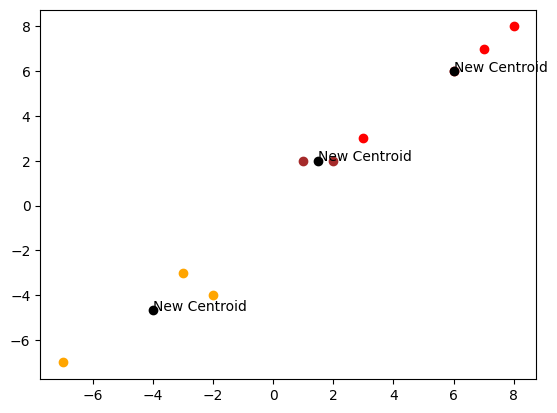
\includegraphics[width=0.6\textwidth]{images/T5_first_iteration.png}
    \caption{Graph after first k-means clustering iteration}
\end{figure}

The second iteration which also the last iteration has assigned the following points to each centroids

\begin{itemize}
    \item Assign (1, 2) to Centroid: (1.5, 2.0)
    \item Assign (3, 3) to Centroid: (1.5, 2.0)
    \item Assign (2, 2) to Centroid: (1.5, 2.0)
    \item Assign (8, 8) to Centroid: (6.0, 6.0)
    \item Assign (6, 6) to Centroid: (6.0, 6.0)
    \item Assign (7, 7) to Centroid: (6.0, 6.0)
    \item Assign (-3, -3) to Centroid: (-4.0, -4.666666666666667)
    \item Assign (-2, -4) to Centroid: (-4.0, -4.666666666666667)
    \item Assign (-7, -7) to Centroid: (-4.0, -4.666666666666667)
\end{itemize}

And we get new three centroids as following point (purple dot)

\begin{itemize}
    \item New Centroid: (7.0, 7.0)
    \item New Centroid: (2.0, 2.3333333333333335)
    \item New Centroid: (-4.0, -4.666666666666667)
\end{itemize}

\begin{figure}[ht]
    \centering
    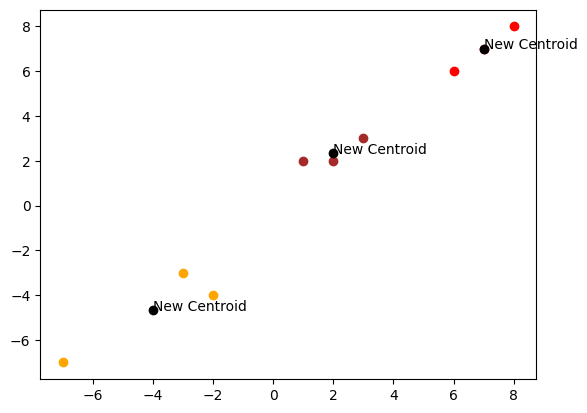
\includegraphics[width=0.6\textwidth]{images/T5_second_iteration.png}
    \caption{Graph after second k-means clustering iteration}
\end{figure}

\subsection{T6}

After changing the starting points to (-3, -3), (2, 2), (-7, -7) the following points are assigned to starting point

\begin{itemize}
    \item Assign (1, 2) to Centroid: (2, 2)
    \item Assign (3, 3) to Centroid: (2, 2)
    \item Assign (2, 2) to Centroid: (2, 2)
    \item Assign (8, 8) to Centroid: (2, 2)
    \item Assign (6, 6) to Centroid: (2, 2)
    \item Assign (7, 7) to Centroid: (2, 2)
    \item Assign (-3, -3) to Centroid: (-3, -3)
    \item Assign (-2, -4) to Centroid: (-3, -3)
    \item Assign (-7, -7) to Centroid: (-7, -7)
\end{itemize}

And we get new three centroids as following point (purple dot)

\begin{itemize}
    \item New Centroid: (-2.5, -3.5)
    \item New Centroid: (4.5, 4.666666666666667)
    \item New Centroid: (-7.0, -7.0)
\end{itemize}

we also see that centroid points have converged to stable point faster than T5 question 
and cluster is more grouping compared to T5 question

\begin{figure}[ht]
    \centering
    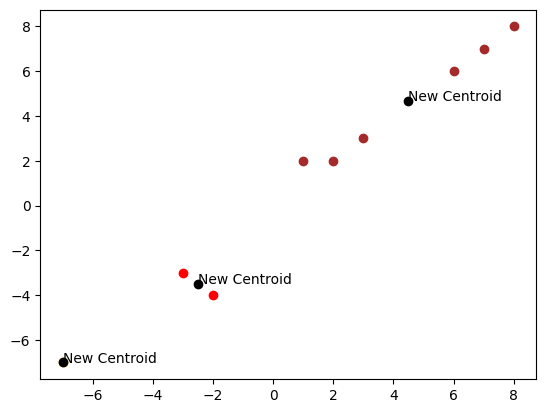
\includegraphics[width=0.6\textwidth]{images/T6_k_means.png}
    \caption{Graph after running k-means clustering}
\end{figure}

\subsection{T7}

I think the starting point from T5 is better than T6. I have measured "goodness" 
by using arithmetic mean of the euclidean distance between centroid and point in each cluster

\noindent If we consider the arithmetic mean for T5 and T6 we will get that

\begin{itemize}
    \item T5: Arithmetic mean of distance = 1.4744582139275695
    \item T6: Arithmetic mean of distance = 2.4413195239469854
\end{itemize}

which means the starting point from T6 question causes more sparse result cluster compared to starting point from T5 question

\pagebreak
\section{My heart will go on}
\subsection{Jupyter Notebook (T8-T13,OT3,OT4)}

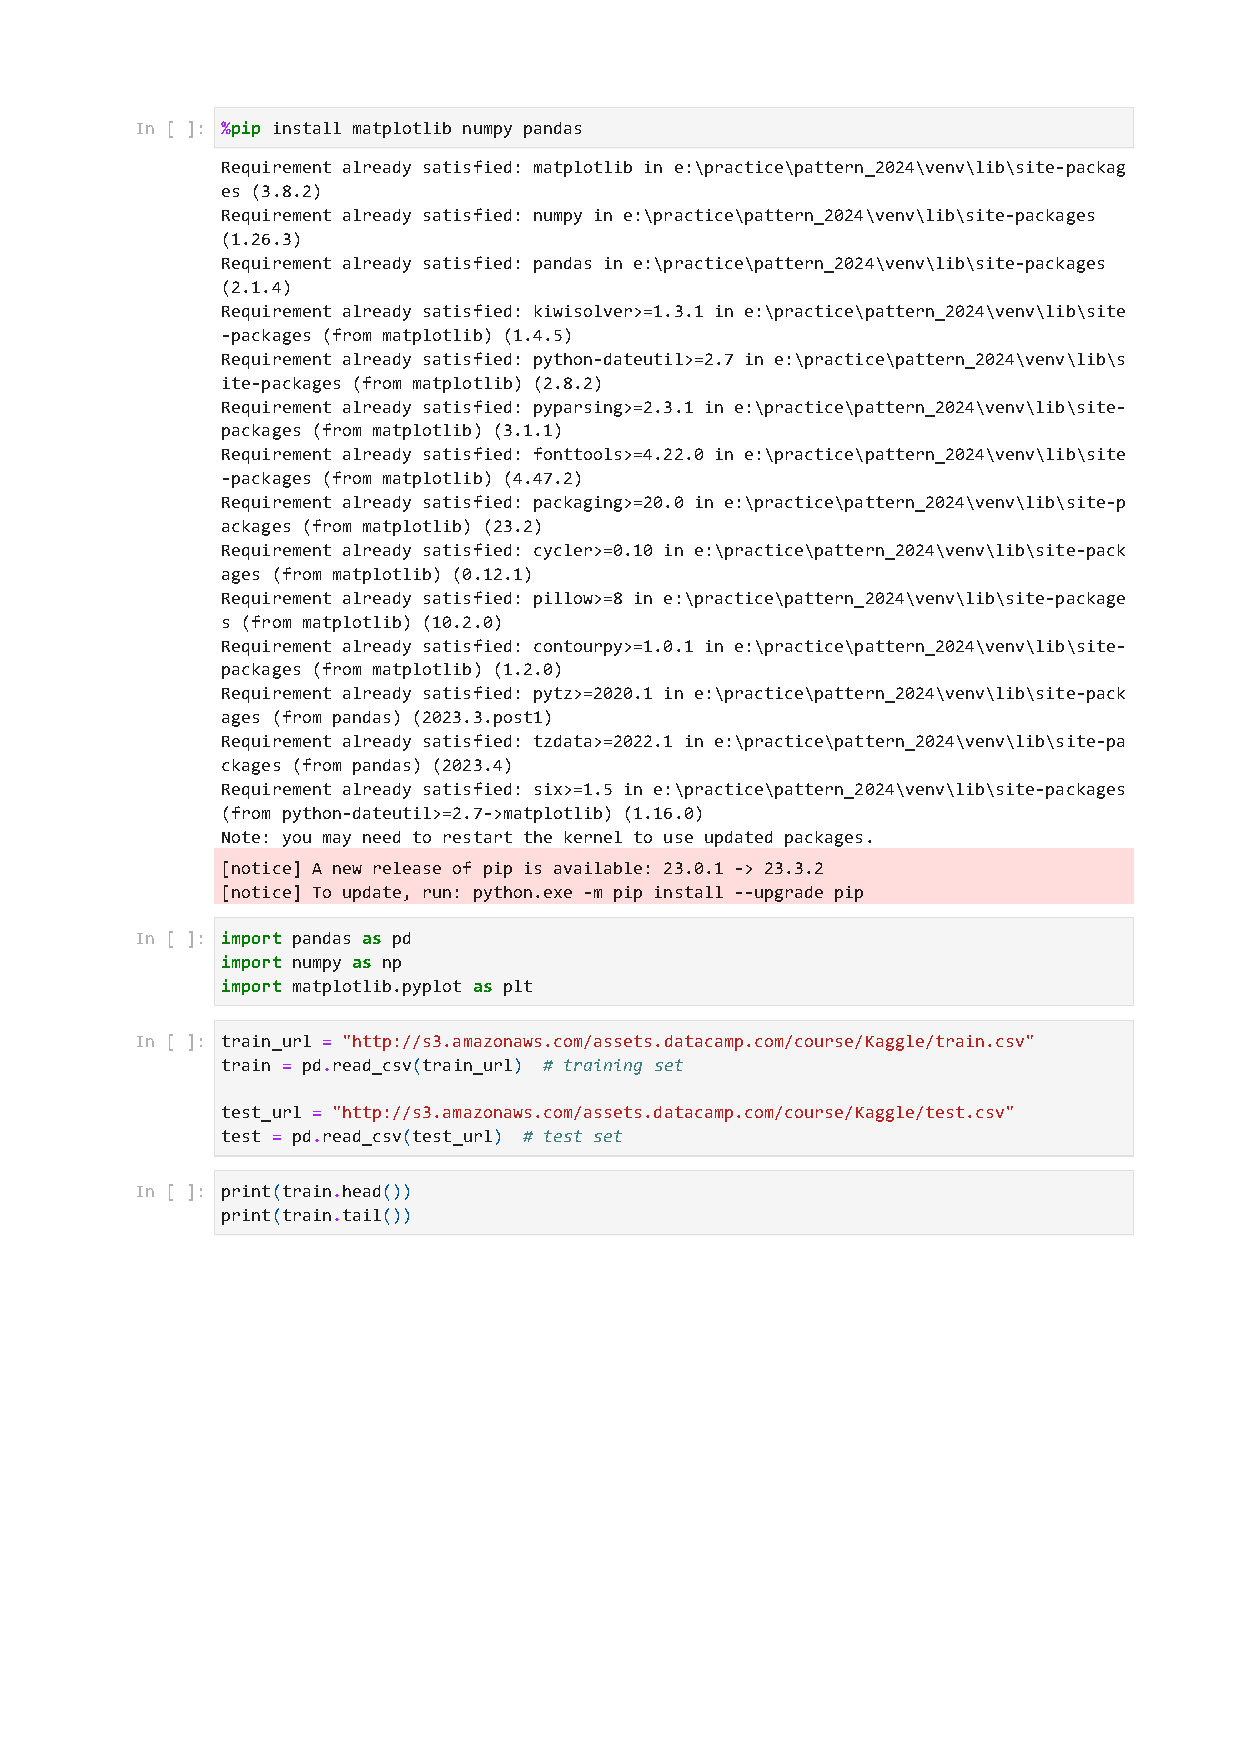
\includepdf[pages=-]{pdf/HW_1_Notebook_Regression.pdf}
\pagebreak

\subsection{OT5}

Show that $\nabla_{A}trAB = B^{T}$

Because $tr$ can be used only if $AB$ is a square matrix so assume that $A$ is a matrix size $N * M$ and $B$ is a matrix size $M * N$

\begin{equation}
    \begin{split}
        X &= \nabla_{A}trAB \\
        X_{i,j} &= \frac{\partial \sum_{a=1}^{a=N} \sum_{b=1}^{b=M} A_{a,b}B_{b,a}}{\partial A_{i,j}} \\
                &= \frac{\partial A_{i,j} B_{j,i}}{\partial A_{i,j}} \\
                &= B_{j,i} \\
        \therefore \nabla_{A}trAB = X &= B^{T}
    \end{split}
\end{equation}

\subsection{OT6}

Show that $\nabla_{A^{T}}f(A) = (\nabla_{A}f(A))^{T}$

Assume that $A$ is a matrix size $N * M$ and let $X = \nabla_{A}f(A)$, $Y = \nabla_{A^{T}}f(A)$

\begin{equation}
    \begin{split}
        Y_{i,j} &= \frac{\partial f(A)}{\partial A_{j,i}} \\
                &= X_{j,i} \\
        \therefore \nabla_{A^{T}}f(A) = Y &= X^{T} = (\nabla_{A}f(A))^{T}
    \end{split}
\end{equation}

\end{document}